\documentclass[tikz,crop]{standalone}

\usepackage{tikz}
\usetikzlibrary{calc, positioning, backgrounds}

\begin{document}
    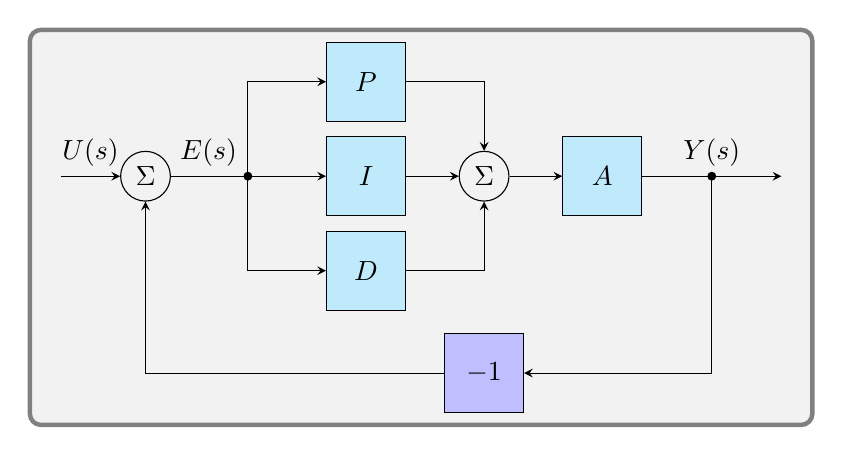
\begin{tikzpicture}[
        auto,
        >=stealth,
        on grid,
        block/.style={draw, rectangle, minimum height=10mm, minimum width=10mm, inner sep=1mm},
        sum/.style={draw, circle, inner sep=1mm},
        dot/.style={anchor=base, fill=black, circle, inner sep=0.4mm},
        show background rectangle,
        background rectangle/.style={fill=gray!10, rounded corners, ultra thick,draw=gray},
    ]
        \node (input) at (0,0) {};
        \node [sum, right=12mm of input] (sum) {$\Sigma$};
        \node [block, right=28mm of sum, fill=cyan!25] (ki) {$I$};
        \node [block, above=12mm of ki, fill=cyan!25] (kp) {$P$};
        \node [block, below=12mm of ki, fill=cyan!25] (kd) {$D$};
        \node [sum, right=15mm of ki] (pid_sum) {$\Sigma$};
        \node [block, right=15mm of pid_sum, fill=cyan!25] (plant) {$A$};
        \node [right=24mm of plant] (output) {};
        \node [block, below=25mm of pid_sum, fill=blue!25] (gain) {$-1$};

        \draw [->] (input) -- node[above]{$U(s)$} (sum);
        \node[above] at ($(sum)+(8mm,0)$) {$E(s)$};
        \draw [->] (sum) -- (ki);
        \draw [->] (sum) ++ (13mm,0) |- (kp) node[dot, at start]{};
        \draw [->] (sum) ++ (13mm,0) |- (kd);
        \draw [->] (kp) -| (pid_sum);
        \draw [->] (ki) -- (pid_sum);
        \draw [->] (kd) -| (pid_sum);
        \draw [->] (pid_sum) -- (plant);
        \draw [->] (plant) -- node[above, name=out]{$Y(s)$} (output);
        \draw [->] (out) |- (gain) node[dot, at start]{};
        \draw [->] (gain) -| (sum);
    \end{tikzpicture}
\end{document}
